\documentclass[11pt]{amsart}

\usepackage[margin=1.3in]{geometry}

\usepackage{amssymb}
\usepackage{amsthm,amsmath}
\usepackage{mathtools}
\usepackage{graphicx}
\usepackage{xcolor}
\usepackage{enumitem}

\usepackage{tikz}
\usetikzlibrary{arrows.meta,calc}
\usepackage{float}

% A little extra breathing room around figures.
\setlength{\textfloatsep}{30pt plus 6pt minus 4pt}
\setlength{\intextsep}{28pt plus 6pt minus 4pt}
\setlength{\abovecaptionskip}{13pt}
\setlength{\belowcaptionskip}{4pt}

\usepackage{hyperref}
\hypersetup{
    colorlinks=true,
    linkcolor=blue!50!black,
    citecolor=blue!50!black,
    urlcolor=blue!50!black,
    pdftitle={Structural properties of Schnyder woods on planar and toroidal triangulations},
    pdfauthor={Octavian Vasile}
}

% Display "Abstract" as a centered heading above the abstract text.
\usepackage{etoolbox}
\patchcmd{\abstract}
  {\item[\hskip\labelsep\scshape\abstractname.]}
  {\item[]\leavevmode\par\centerline{\scshape\abstractname}\par\smallskip}
  {}{}

% Colors used in the figures.
\definecolor{ColZero}{RGB}{65,65,255}
\definecolor{ColOne}{RGB}{255,65,65}
\definecolor{ColTwo}{RGB}{0,0,0}

% Notation.
\newcommand{\Zthree}{\{0,1,2\}}
\newcommand{\indeg}{\operatorname{indeg}}
\newcommand{\out}{\operatorname{out}}
\newcommand{\inn}{\operatorname{in}}

% Theorem environments.
\theoremstyle{plain}
\newtheorem{theorem}{Theorem}
\newtheorem{proposition}[theorem]{Proposition}
\newtheorem{lemma}[theorem]{Lemma}
\newtheorem{corollary}[theorem]{Corollary}

\theoremstyle{definition}
\newtheorem{definition}[theorem]{Definition}

\theoremstyle{remark}
\newtheorem{remark}[theorem]{Remark}


\begin{document}

\title[Schnyder woods on planar and toroidal triangulations]%
      {Structural properties of Schnyder woods on planar and toroidal triangulations}

\author{Octavian Vasile}

\dedicatory{%
  \normalfont
  \'Ecole Polytechnique, France\\
  \texttt{octavian.vasile@polytechnique.edu}%
}

\date{}

\begin{abstract}
The defining feature of a Schnyder wood is a single rule imposed locally at each vertex, and it is natural to ask how much global structure this rule already determines. We study this question for planar and toroidal triangulations, where the same local condition leads to different behaviors. In the plane, it organizes the edges into three rooted spanning trees. On the torus, where no roots are distinguished, these trees are replaced by monochromatic functional digraphs, each weak component carrying exactly one directed cycle, and the leaves are replaced by sources, namely vertices with no incoming edge of a fixed color.
The first part of the paper proves face counting identities forced only by the local rule. These identities reveal a common mechanism behind the planar and toroidal settings, despite the different global shape of the color classes. In the toroidal case, we combine this identity with an edge disjointness argument for tri-colored faces to obtain a linear lower bound on the total number of sources of any minimal toroidal Schnyder wood.
The final part concerns balanced toroidal Schnyder woods. Using their dual acyclicity property, we give a direct proof that every balanced toroidal Schnyder wood contains both a clockwise and a counterclockwise oriented contractible triangle. The proof uses leftmost walks, face labels, and an Euler count on a maximal labeled region, illustrating how a global hypothesis can turn local successor rules into topological information.





\end{abstract}

\maketitle

\setcounter{tocdepth}{1}
\begingroup
\hypersetup{linkcolor=black}
\tableofcontents
\endgroup

\section{Introduction}
\label{sec:introduction}

Schnyder woods are a classical combinatorial structure on triangulated planar graphs. They assign directions and colors to the edges of a triangulation according to a local rule. In the planar case, together with the usual boundary convention, this local rule produces three rooted spanning trees. This viewpoint originates in early work on planar graph dimension and grid embeddings~\cite{schnyder1989,schnyder1990}, and was later developed through the theory of graph orientations and distributive lattices~\cite{felsner2001,felsner2004}.

The toroidal setting has a different flavor. Since there is no distinguished outer face, there is no canonical choice of roots. The local Schnyder rule becomes fully symmetric: for each color, every vertex has exactly one outgoing edge. Consequently, the monochromatic subgraphs are not rooted trees but functional directed graphs, each weak component containing a directed cycle. Thus passing from the plane to the torus replaces rooted structure by cyclic structure, which changes both the statements and the methods of proof.

Schnyder woods on higher-genus triangulated surfaces have also been studied, extending the planar theory to closed orientable surfaces and applying it to traversal and encoding algorithms~\cite{castelli-fusy-lewiner2009}. In the toroidal setting, a symmetric definition for toroidal maps was introduced, and such Schnyder woods were shown to exist exactly for essentially $3$-connected toroidal maps~\cite{goncalves-leveque2014}. The balanced, or HTC, class of toroidal Schnyder woods was later studied, and the existence of both a clockwise and a counterclockwise oriented contractible triangle was established in this setting~\cite{despre-goncalves-leveque2017}.

A second motivation comes from the planar theory of leaf counts. The leaves of the three rooted trees of a planar Schnyder wood are natural structural parameters, and lower bounds on their number have recently been obtained, both for $3$-connected planar maps and, in the sharper triangulated case, a bound of $(3n+3)/2$ on the total number of leaves of a Schnyder wood of a plane triangulation on $n$ vertices~\cite{ortlieb-schmidt}. On the torus the role played by the leaves of the three rooted trees is played instead by the \emph{sources} of the three monochromatic functional digraphs: as recalled above, these digraphs are no longer rooted trees but functional graphs whose components each carry a unique directed cycle, so there are no leaves to count and the sources become the natural substitute. It is therefore natural to seek the toroidal analogue of such a leaf bound, namely a lower bound on the total number of sources; the lower bound of Section~\ref{sec:toroidal-lower-bound} is the outcome of pursuing this analogy.

The paper has two main contributions. The first is a toroidal source--face identity and the lower bound it implies. We show that, for each color, the number of sources in the corresponding monochromatic functional digraph equals the number of triangular faces carrying exactly two edges of that color (Theorem~\ref{thm:toroidal-source-face}). This is the toroidal analogue of the planar leaf--face identity (Theorem~\ref{thm:planar-leaf-identity}), which we prove first as a model case. Combined with an edge-disjointness argument for tri-colored faces, the identity yields in Section~\ref{sec:toroidal-lower-bound} a linear lower bound of at least $\frac{6n-6}{5}$ sources for a triangulation on $n$ vertices (Theorem~\ref{thm:toroidal-lower-bound}). The second contribution is a new proof of a known result (Theorem~\ref{thm:balanced-oriented-triangles}): every balanced toroidal Schnyder wood contains both a clockwise and a counterclockwise oriented contractible triangle~\cite{despre-goncalves-leveque2017}. Our proof is direct and combinatorial, using a leftmost-walk construction, face labels, and an Euler-characteristic count on a maximal labeled region. Its only global input is the dual acyclicity supplied by balancedness.


\section{Preliminaries}
\label{sec:prelim}

Throughout the paper, graphs are considered together with a fixed embedding on a compact orientable surface. Following standard terminology, such an embedded graph is called a \emph{map}. Thus a map consists of a finite graph embedded in a compact surface in such a way that every connected component of the complement is homeomorphic to an open disk. These connected components are called the \emph{faces} of the map. A map is \emph{simple} if its underlying graph has no loops and no multiple edges.

A \emph{plane triangulation} is a simple map embedded in the sphere, with one face distinguished as the outer face, such that every face has degree $3$. The boundary of the outer face is denoted by $r_0 r_1 r_2$, with the vertices listed counterclockwise.

A \emph{simple toroidal triangulation} is a simple map embedded on the torus such that every face has degree $3$. If such a triangulation has $n$ vertices, $m$ edges, and $f$ faces, then Euler's formula on the torus and double-counting edge--face incidences give
\[
  n-m+f = 0, \qquad 3f = 2m.
\]
Consequently $m = 3n$ and $f = 2n$.

An \emph{angle} is an incidence between a vertex and a face. Equivalently, it is the sector determined by two consecutive edge-ends in the cyclic order around the vertex.

A closed walk on the torus is called \emph{contractible} if it can be continuously shrunk to a point on the surface. A simple closed curve on the torus is contractible exactly when it bounds a disk.

We shall use the following standard observation. If a directed closed walk on the
torus is non-contractible, then one of the directed simple cycles contained in it is
also non-contractible. Indeed, whenever the walk repeats a vertex, we may split it at
that vertex into shorter directed closed walks. Repeating this process decomposes the
walk into directed simple cycles. If all these simple cycles were contractible, then
they could be contracted one after another, and their concatenation would also contract
to a point. Hence at least one of them is non-contractible.

Throughout the paper, the colors are taken from $\{0, 1, 2\}$, and all color indices are taken modulo $3$.

When an edge is directed and colored, an endpoint of the edge is called the \emph{tail} if the edge is directed away from it, and the \emph{head} if the edge is directed toward it. At the tail the edge is \emph{outgoing}; at the head it is \emph{incoming}. In the planar boundary convention below, an outer boundary edge carries two opposite directed colored copies. For a directed graph $D$, the indegree of a vertex $v$ is denoted by $\indeg_D(v)$.

\begin{definition}
\label{def:local-schnyder}
Let $v$ be a vertex incident with directed colored edges using colors in $\Zthree$. We say that $v$ satisfies the \emph{local Schnyder property} if, in counterclockwise order around $v$, the incident directed colored edges occur in six consecutive blocks
\[
  \out(0),\ \inn(2),\ \out(1),\ \inn(0),\ \out(2),\ \inn(1),
\]
where each $\out(i)$ block consists of exactly one outgoing edge of color $i$, and each $\inn(i)$ block consists of zero or more incoming edges of color $i$. See Figure~\ref{fig:local-schnyder}.
\end{definition}

\begin{figure}[H]
\centering
\begin{tikzpicture}[
  scale=1.78,
  >={Stealth[length=2.4mm,width=1.8mm,inset=0.5mm]},
  line cap=round,
  line join=round,
  every node/.style={font=\small}
]
  \coordinate (v) at (0,0);

  % Three outgoing edges
  \draw[->, line width=0.9pt, ColZero] (v) -- (  0:1.9);
  \draw[->, line width=0.9pt, ColOne]  (v) -- (120:1.9);
  \draw[->, line width=0.9pt, ColTwo]  (v) -- (240:1.9);

  % Incoming edges, two per in-block
  \draw[->, line width=0.55pt, ColTwo]  ( 50:1.9) -- ( 50:0.25);
  \draw[->, line width=0.55pt, ColTwo]  ( 75:1.9) -- ( 75:0.25);
  \draw[->, line width=0.55pt, ColZero] (170:1.9) -- (170:0.25);
  \draw[->, line width=0.55pt, ColZero] (195:1.9) -- (195:0.25);
  \draw[->, line width=0.55pt, ColOne]  (290:1.9) -- (290:0.25);
  \draw[->, line width=0.55pt, ColOne]  (315:1.9) -- (315:0.25);

  % Central vertex
  \filldraw[fill=black] (v) circle (1.4pt);

  % Block labels
  \node[ColZero, right]       at (  0:2.15) {$\out(0)$};
  \node[ColTwo,  above right] at ( 60:2.05) {$\inn(2)$};
  \node[ColOne,  above left]  at (120:2.15) {$\out(1)$};
  \node[ColZero, left]        at (180:2.15) {$\inn(0)$};
  \node[ColTwo,  below left]  at (240:2.15) {$\out(2)$};
  \node[ColOne,  below right] at (300:2.05) {$\inn(1)$};
\end{tikzpicture}
\caption{The local Schnyder property at $v$.}
\label{fig:local-schnyder}
\end{figure}

\begin{lemma}[\cite{felsner2004}]
\label{lem:separation}
Fix $i \in \Zthree$. At a vertex satisfying the local Schnyder property, the outgoing edge of color $i$ is not consecutive, in the cyclic order around the vertex, to any incoming edge of color $i$.
\end{lemma}

\begin{proof}
If the incoming block of color $i$ is empty, there is nothing to prove. Otherwise, by Definition~\ref{def:local-schnyder}, the incoming block of color $i$ lies between the outgoing edges of colors $i+1$ and $i-1$. Therefore the outgoing edge of color $i$ and the incoming block of color $i$ are separated in the cyclic order by outgoing edges of the other two colors. Hence the outgoing edge of color $i$ cannot be consecutive to an incoming edge of color $i$.
\end{proof}


\section{Planar Schnyder woods of triangulations}
\label{sec:planar}

\begin{definition}
\label{def:planar-schnyder}
Let $G$ be a plane triangulation whose outer face is $r_0 r_1 r_2$, listed counterclockwise. A \emph{planar Schnyder wood} of $G$ consists of an orientation and coloring of the edges of $G$, together with one auxiliary half-edge $h_i$ at each outer vertex $r_i$, satisfying the following conditions.
\begin{enumerate}[label=\textup{(P\arabic*)}]
  \item Every internal edge is directed and colored exactly once.
  \item If an internal edge is incident with the outer vertex $r_i$, then it is directed toward $r_i$ and has color $i$.
  \item Each outer edge $r_i r_j$ carries two opposite directed colored copies: the copy directed toward $r_i$ has color $i$, and the copy directed toward $r_j$ has color $j$.
  \item The half-edge $h_i$ is incident with $r_i$, is directed into the outer face, and has color $i$.
  \item Every vertex satisfies the local Schnyder property, where at $r_i$ the half-edge $h_i$ is the outgoing edge of color $i$.
  \item There is no directed monochromatic cycle supported by the edges of $G$.
\end{enumerate}
\end{definition}

This is the standard suspension convention for planar Schnyder woods of triangulations. The auxiliary half-edge $h_i$ is only used to complete the local rotation at the outer vertex $r_i$; it is not an edge of $G$ and is not incident with any internal face. Similarly, the two directed copies on an outer edge are used only for the two endpoint angles of the unique internal face incident with that outer edge. For general $3$-connected planar maps, one uses the corresponding generalized definition with suspensions; see Felsner~\cite{felsner2001,felsner2004}.

\begin{figure}[ht]
\centering
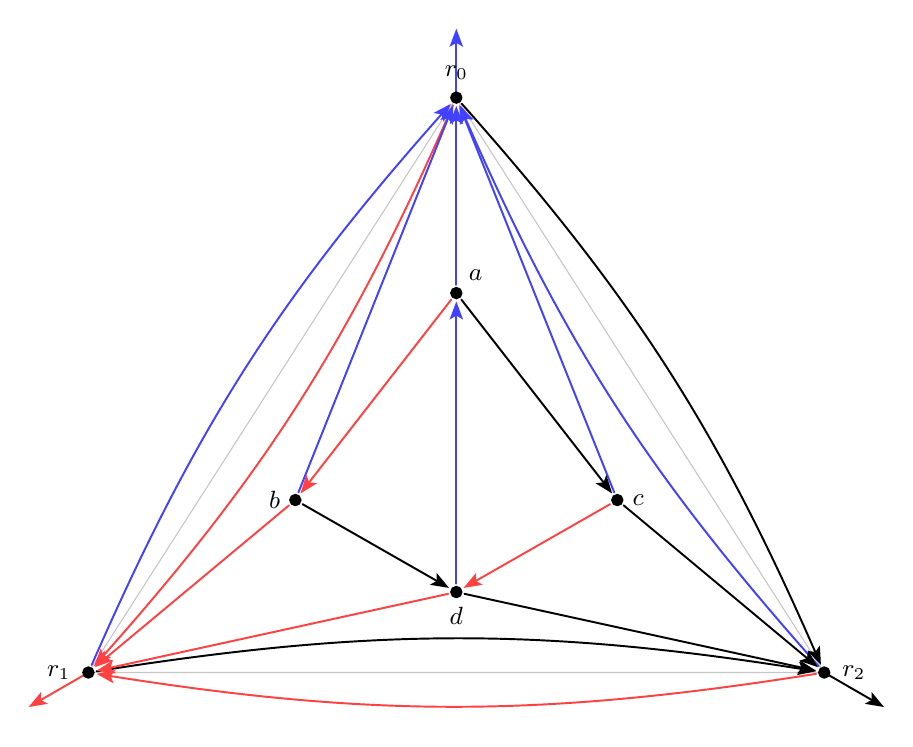
\begin{tikzpicture}[
  scale=1.46,
  >={Stealth[length=2.3mm,width=1.7mm,inset=0.5mm]},
  line cap=round,
  line join=round,
  every node/.style={font=\small}
]
  \coordinate (r0) at ( 0   , 3   );
  \coordinate (r1) at (-3.2 ,-2   );
  \coordinate (r2) at ( 3.2 ,-2   );
  \coordinate (a)  at ( 0   , 1.3 );
  \coordinate (b)  at (-1.4 ,-0.5 );
  \coordinate (c)  at ( 1.4 ,-0.5 );
  \coordinate (d)  at ( 0   ,-1.3 );

  % Outer triangle (faint backbone)
  \draw[gray!45, line width=0.4pt] (r0) -- (r1) -- (r2) -- cycle;

  % Outer edges as two opposite directed copies (slight bend separates them)
  \draw[->, line width=0.7pt, ColZero, shorten >=3pt, shorten <=3pt] (r1) to[bend left=9] (r0);
  \draw[->, line width=0.7pt, ColOne,  shorten >=3pt, shorten <=3pt] (r0) to[bend left=9] (r1);
  \draw[->, line width=0.7pt, ColOne,  shorten >=3pt, shorten <=3pt] (r2) to[bend left=9] (r1);
  \draw[->, line width=0.7pt, ColTwo,  shorten >=3pt, shorten <=3pt] (r1) to[bend left=9] (r2);
  \draw[->, line width=0.7pt, ColTwo,  shorten >=3pt, shorten <=3pt] (r0) to[bend left=9] (r2);
  \draw[->, line width=0.7pt, ColZero, shorten >=3pt, shorten <=3pt] (r2) to[bend left=9] (r0);

  % Half-edges at outer vertices
  \draw[->, line width=0.7pt, ColZero] (r0) -- ($(r0)+( 90:0.6)$);
  \draw[->, line width=0.7pt, ColOne]  (r1) -- ($(r1)+(210:0.6)$);
  \draw[->, line width=0.7pt, ColTwo]  (r2) -- ($(r2)+(330:0.6)$);

  % Tree 0 (color 0, oriented toward r_0)
  \draw[->, line width=0.7pt, ColZero, shorten >=3pt, shorten <=3pt] (a) -- (r0);
  \draw[->, line width=0.7pt, ColZero, shorten >=3pt, shorten <=3pt] (b) -- (r0);
  \draw[->, line width=0.7pt, ColZero, shorten >=3pt, shorten <=3pt] (c) -- (r0);
  \draw[->, line width=0.7pt, ColZero, shorten >=3pt, shorten <=3pt] (d) -- (a);

  % Tree 1 (color 1, oriented toward r_1)
  \draw[->, line width=0.7pt, ColOne, shorten >=3pt, shorten <=3pt] (b) -- (r1);
  \draw[->, line width=0.7pt, ColOne, shorten >=3pt, shorten <=3pt] (d) -- (r1);
  \draw[->, line width=0.7pt, ColOne, shorten >=3pt, shorten <=3pt] (a) -- (b);
  \draw[->, line width=0.7pt, ColOne, shorten >=3pt, shorten <=3pt] (c) -- (d);

  % Tree 2 (color 2, oriented toward r_2)
  \draw[->, line width=0.7pt, ColTwo, shorten >=3pt, shorten <=3pt] (c) -- (r2);
  \draw[->, line width=0.7pt, ColTwo, shorten >=3pt, shorten <=3pt] (d) -- (r2);
  \draw[->, line width=0.7pt, ColTwo, shorten >=3pt, shorten <=3pt] (a) -- (c);
  \draw[->, line width=0.7pt, ColTwo, shorten >=3pt, shorten <=3pt] (b) -- (d);

  % Vertices and labels
  \foreach \pt in {r0, r1, r2, a, b, c, d}{
    \filldraw[fill=black] (\pt) circle (1.4pt);
  }
  \node[above=3pt]       at (r0) {$r_0$};
  \node[left=3pt]        at (r1) {$r_1$};
  \node[right=3pt]       at (r2) {$r_2$};
  \node[above right=1pt] at (a)  {$a$};
  \node[left=2pt]        at (b)  {$b$};
  \node[right=2pt]       at (c)  {$c$};
  \node[below=2pt]       at (d)  {$d$};
\end{tikzpicture}
\caption{A planar Schnyder wood on a $7$-vertex triangulation.}
\label{fig:planar-schnyder-example}
\end{figure}

For $i \in \Zthree$, let $T_i$ be the directed graph formed by the color-$i$ edges supported on edges of $G$. The auxiliary half-edge $h_i$ is not included in $T_i$.

\begin{lemma}[\cite{schnyder1989}]
\label{lem:planar-tree-property}
For every $i \in \Zthree$, the directed graph $T_i$ is a spanning tree oriented toward the root $r_i$.
\end{lemma}

\begin{proof}
By Definition~\ref{def:planar-schnyder}, the root $r_i$ has no outgoing color-$i$ edge supported by an edge of $G$, since its only outgoing color-$i$ edge is the half-edge $h_i$. Every other vertex has exactly one outgoing color-$i$ edge supported by an edge of $G$: for an internal vertex this is the unique color-$i$ outgoing edge required by the local Schnyder property, and for an outer vertex $r_j$ with $j \neq i$ this is the copy of the outer edge $r_j r_i$ directed toward $r_i$. Hence $T_i$ has exactly $n-1$ directed edges.

Starting from any vertex different from $r_i$ and repeatedly following the unique outgoing color-$i$ edge, one of two things happens: either the path reaches $r_i$, or some vertex repeats. In the second case, the repeated segment gives a directed monochromatic cycle supported by edges of $G$, contradicting Definition~\ref{def:planar-schnyder}. Thus every vertex reaches $r_i$. Therefore the underlying undirected graph of $T_i$ is connected; a connected graph on $n$ vertices with $n-1$ edges is a tree. Since every vertex different from $r_i$ reaches $r_i$ by following directed edges, this tree is oriented toward $r_i$.
\end{proof}

\begin{lemma}
\label{lem:planar-no-monochromatic-face}
Let $F$ be an internal face of $G$ which is not incident with an outer edge. Then the three edges on the boundary of $F$ are not all of the same color.
\end{lemma}

\begin{proof}
Suppose that the three boundary edges of $F$ all have color $i$. Since $F$ is not incident with an outer edge, all three of its boundary edges are internal edges and hence are each directed exactly once. Each of the three boundary edges has both endpoints on $\partial F$, so its tail lies on $\partial F$; the total number of outgoing color-$i$ incidences along $\partial F$ is therefore $3$.

At any vertex there is at most one outgoing edge of color $i$. Since $\partial F$ has three vertices and the total number of outgoing color-$i$ incidences along $\partial F$ is $3$, each vertex of $F$ is the tail of exactly one boundary edge of $F$. Therefore the boundary of $F$ is a directed monochromatic cycle, contradicting Definition~\ref{def:planar-schnyder}. Hence $F$ is not monochromatic.
\end{proof}


\section{A planar leaf identity}
\label{sec:planar-id}

Throughout this section let $G$ be a plane triangulation with $n \ge 4$ vertices and outer face $r_0 r_1 r_2$, equipped with a planar Schnyder wood. For $i \in \Zthree$ and $v \in V(G)$, define
\[
  c_i(v) := \indeg_{T_i}(v),
  \qquad
  l_i := \#\{v \in V(G) : c_i(v) = 0\}.
\]
By Lemma~\ref{lem:planar-tree-property}, $T_i$ is a rooted tree oriented toward $r_i$, so $l_i$ counts the leaves of $T_i$.

An internal face is called \emph{boundary-adjacent} if one of its three sides is an edge of the outer face. Since the outer face is the triangle $r_0 r_1 r_2$, each of its three edges is incident with exactly one internal face. These three internal faces are distinct when $n \ge 4$. Indeed, if an internal triangular face were incident with two outer edges, then its third side would necessarily be the remaining outer edge, so its boundary would be the same triangle $r_0 r_1 r_2$ as the outer face. This would force the graph to be just the outer triangle.

Thus there are exactly three boundary-adjacent internal faces. We denote by $\kappa$ the number of internal faces which are not boundary-adjacent and whose three edge colors are pairwise distinct.

\begin{theorem}
\label{thm:planar-leaf-identity}
For every plane triangulation $G$ with $n \ge 4$ vertices, equipped with a planar Schnyder wood,
\[
  \sum_{i \in \Zthree} l_i \;=\; 2n + 1 - \kappa.
\]
\end{theorem}

\begin{proof}
For a color $i \in \Zthree$, let $B_i$ be the number of angles of internal faces whose two sides are both incoming edges of color $i$. We first express $B_i$ in terms of $l_i$.

Fix $i$, and let $v \in V(G)$. The incoming edges of color $i$ at $v$ form a single contiguous block in the cyclic order around $v$, by the local Schnyder property. Write $c_i(v) = k$. If $k = 0$, there is no pair of consecutive incoming color-$i$ edges at $v$. If $k \ge 1$, the block contains exactly $k-1$ consecutive pairs of incoming color-$i$ edges. Since $G$ is a triangulation, each such pair bounds a unique angle of an internal face, and every angle counted by $B_i$ arises in this way. Note that the outer-face angle at $r_i$ lies between the two outgoing edges of colors $i+1$ and $i-1$ (with the half-edge $h_i$ inside it) rather than between two incoming color-$i$ edges, and that conditions (P2)--(P3) force $c_i(r_j) = 0$ for $j \neq i$, so outer vertices other than $r_i$ contribute nothing to the sum either. Therefore
\[
  B_i
  \;=\;
  \sum_{v \in V(G)} \max\{c_i(v) - 1,\, 0\}
  \;=\;
  \sum_{c_i(v) > 0} \bigl(c_i(v) - 1\bigr).
\]
The tree $T_i$ has $n - 1$ edges, so counting its edges by their heads gives
\[
  \sum_{v \in V(G)} c_i(v) \;=\; n - 1.
\]
Setting $t_i := \#\{v \in V(G) : c_i(v) > 0\}$, we obtain $B_i = (n - 1) - t_i$. Since $l_i = n - t_i$, this yields $B_i = l_i - 1$. Summing over the three colors,
\[
  \sum_{i \in \Zthree} l_i \;=\; 3 + B,
  \qquad B := B_0 + B_1 + B_2.
\]

It remains to compute $B$ by summing over internal faces. A plane triangulation with $n$ vertices has $2n - 5$ internal faces, of which exactly three are boundary-adjacent.

Let $F$ be a boundary-adjacent internal face, with outer edge $r_j r_k$ and third vertex $u$. The edge $u r_j$ is directed toward $r_j$ and has color $j$, and the copy of the outer edge $r_j r_k$ directed toward $r_j$ also has color $j$; these two incoming color-$j$ edges are consecutive around $r_j$ and bound the angle of $F$ at $r_j$. Symmetrically, the edge $u r_k$ and the copy of $r_j r_k$ directed toward $r_k$ form a consecutive pair of incoming color-$k$ edges at $r_k$. The third angle of $F$ is at $u$, where the two incident edges are outgoing of colors $j$ and $k$, and so contribute nothing to $B$. Hence $F$ contributes exactly two angles to $B$.

\begin{figure}[H]
\centering
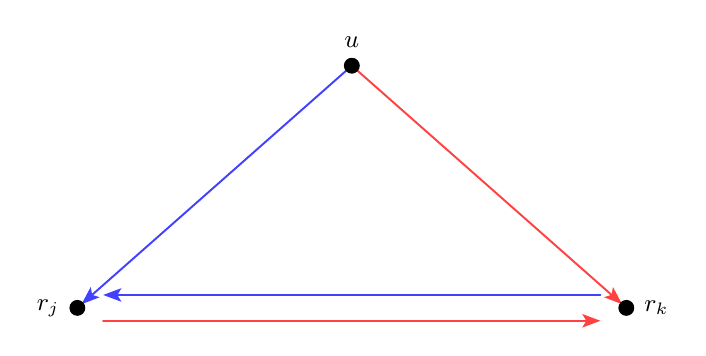
\begin{tikzpicture}[
  scale=2.05,
  >={Stealth[length=2.3mm,width=1.7mm,inset=0.5mm]},
  line cap=round,
  line join=round,
  every node/.style={font=\small}
]
  \coordinate (rj) at (-1.7, 0);
  \coordinate (rk) at ( 1.7, 0);
  \coordinate (u)  at ( 0  , 1.5);

  % Outer edge: two opposite directed copies
  \draw[->, line width=0.7pt, ColZero] ($(rk)+(-0.16, 0.08)$) -- ($(rj)+( 0.16, 0.08)$);
  \draw[->, line width=0.7pt, ColOne]  ($(rj)+( 0.16,-0.08)$) -- ($(rk)+(-0.16,-0.08)$);

  % Inner edges of the face
  \draw[->, line width=0.7pt, ColZero, shorten >=2pt] (u) -- (rj);
  \draw[->, line width=0.7pt, ColOne,  shorten >=2pt] (u) -- (rk);

  \foreach \pt in {rj, rk, u}{
    \filldraw[fill=black] (\pt) circle (1.3pt);
  }

  \node[left=3pt]  at (rj) {$r_j$};
  \node[right=3pt] at (rk) {$r_k$};
  \node[above=3pt] at (u)  {$u$};
\end{tikzpicture}
\caption{A boundary-adjacent face.}
\label{fig:boundary-adjacent-face}
\end{figure}

Now let $F$ be an internal face which is not boundary-adjacent. If the three colors on $F$ are pairwise distinct, then $F$ contributes no angle to $B$. Otherwise, by Lemma~\ref{lem:planar-no-monochromatic-face}, the color multiset on $F$ is $\{i, i, j\}$ for some $i \neq j$. The two color-$i$ edges meet at a unique vertex $v$. They cannot both be outgoing at $v$, because $v$ has at most one outgoing edge of color $i$. They also cannot consist of one outgoing and one incoming color-$i$ edge, by Lemma~\ref{lem:separation}, since the two edges are consecutive around $v$. Therefore both color-$i$ edges are incoming at $v$, and they determine exactly one angle counted by $B_i$. Thus such a face contributes exactly one angle to $B$.

Therefore
\[
  B \;=\; 2 \cdot 3 + \bigl((2n - 5) - 3 - \kappa\bigr) \;=\; 2n - 2 - \kappa,
\]
and consequently
\[
  \sum_{i \in \Zthree} l_i \;=\; 3 + B \;=\; 2n + 1 - \kappa. \qedhere
\]
\end{proof}


\section{Toroidal Schnyder orientations}
\label{sec:toroidal}

\begin{definition}
\label{def:local-toroidal-schnyder}
Let $G$ be a simple toroidal triangulation. A \emph{local toroidal Schnyder orientation} of $G$ is an orientation and coloring of every edge of $G$ with a color in $\Zthree$ such that every vertex satisfies the local Schnyder property of Definition~\ref{def:local-schnyder}.
\end{definition}

\begin{figure}[ht]
\centering
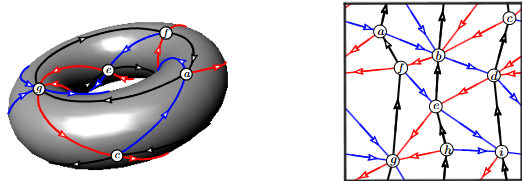
\includegraphics[width=0.85\linewidth]{torus-schnyder-example.png}
\caption{A toroidal Schnyder wood, on the torus and in the plane.}
\label{fig:torus-schnyder-example}
\end{figure}

\begin{lemma}
\label{lem:toroidal-no-monochromatic-face}
No facial triangle of a local toroidal Schnyder orientation is monochromatic.
\end{lemma}

\begin{proof}
Suppose that a facial triangle $F$ were monochromatic of color $i$. Since every edge is oriented and colored exactly once in a local toroidal Schnyder orientation, each of the three boundary edges of $F$ is directed exactly once. Thus the total number of outgoing color-$i$ incidences along $\partial F$ is $3$. Since each vertex has at most one outgoing edge of color $i$, each vertex of $F$ is the tail of exactly one boundary edge of $F$. Thus the boundary of $F$ is a directed monochromatic triangle.

At each vertex of this triangle, the outgoing color-$i$ edge and the incoming color-$i$ edge are consecutive around the vertex, since they bound the corresponding angle of the facial triangle. This contradicts Lemma~\ref{lem:separation}. Therefore $F$ is not monochromatic.
\end{proof}

\begin{figure}[H]
\centering
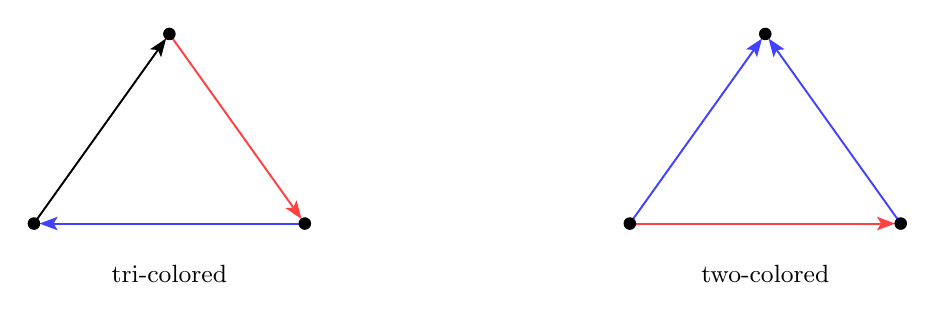
\begin{tikzpicture}[
  scale=1.72,
  >={Stealth[length=2.3mm,width=1.7mm,inset=0.5mm]},
  line cap=round,
  line join=round,
  every node/.style={font=\small}
]
  % Tri-colored face
  \begin{scope}[xshift=-2.2cm]
    \coordinate (a) at (-1, 0);
    \coordinate (b) at ( 1, 0);
    \coordinate (c) at ( 0, 1.4);
    \draw[->, line width=0.7pt, ColZero, shorten >=2pt] (b) -- (a);
    \draw[->, line width=0.7pt, ColTwo,  shorten >=2pt] (a) -- (c);
    \draw[->, line width=0.7pt, ColOne,  shorten >=2pt] (c) -- (b);
    \foreach \pt in {a,b,c}{\filldraw[fill=black] (\pt) circle (1.2pt);}
    \node[below=4pt] at (0,-0.15) {tri-colored};
  \end{scope}

  % Two-colored face (one repeated color)
  \begin{scope}[xshift=2.2cm]
    \coordinate (a) at (-1, 0);
    \coordinate (b) at ( 1, 0);
    \coordinate (c) at ( 0, 1.4);
    \draw[->, line width=0.7pt, ColZero, shorten >=2pt] (a) -- (c);
    \draw[->, line width=0.7pt, ColZero, shorten >=2pt] (b) -- (c);
    \draw[->, line width=0.7pt, ColOne,  shorten >=2pt] (a) -- (b);
    \foreach \pt in {a,b,c}{\filldraw[fill=black] (\pt) circle (1.2pt);}
    \node[below=4pt] at (0,-0.15) {two-colored};
  \end{scope}
\end{tikzpicture}
\caption{The two color patterns on a face.}
\label{fig:face-types}
\end{figure}

For $i \in \Zthree$, let $G_i$ be the directed subgraph formed by the color-$i$ edges of $G$. Since each color-$i$ edge is directed only once, $G_i$ is a directed graph in the usual sense, and each vertex has exactly one outgoing edge in $G_i$.

\begin{lemma}[\cite{goncalves-leveque2014}]
\label{lem:monochromatic-components}
For every $i \in \Zthree$, every weakly connected component of $G_i$ contains exactly one directed cycle.
\end{lemma}

\begin{proof}
Fix $i \in \Zthree$, and let $C$ be a weakly connected component of $G_i$. Each vertex of $C$ has exactly one outgoing edge of color $i$, and the head of this edge also lies in $C$. Hence the restriction of $G_i$ to $C$ has exactly $|V(C)|$ directed edges. Since $G$ is simple, so is the underlying undirected graph of $C$; its cyclomatic number is therefore
\[
  |E(C)| - |V(C)| + 1 \;=\; 1.
\]
Thus the underlying undirected graph of $C$ has exactly one cycle.

Since $C$ is finite and every vertex has outdegree $1$, repeatedly following outgoing edges from any vertex eventually repeats a vertex and produces a directed cycle. This directed cycle is supported by the unique undirected cycle of $C$, so it is the only directed cycle in $C$.
\end{proof}

This is the toroidal counterpart of the rooted-tree property in the plane (Lemma~\ref{lem:planar-tree-property}): on the torus there is no distinguished root for the color class $G_i$ to flow into, and each weak component instead absorbs into a unique directed cycle. We record this lemma for structural context, and it is the underlying reason why the relevant counting object on the torus is the number of \emph{sources} $z_i$ rather than the number of leaves.

\begin{figure}[ht]
\centering
\begin{tikzpicture}[
  scale=1.68,
  >={Stealth[length=2.3mm,width=1.7mm,inset=0.5mm]},
  line cap=round,
  line join=round,
  every node/.style={font=\small}
]
  % The cycle
  \coordinate (c1) at ( 0  , 0);
  \coordinate (c2) at ( 1.6, 0);
  \coordinate (c3) at ( 2.0, 1.3);
  \coordinate (c4) at ( 0.6, 1.8);
  \coordinate (c5) at (-0.6, 1.0);

  \draw[->, line width=0.75pt, shorten >=2pt] (c1) -- (c2);
  \draw[->, line width=0.75pt, shorten >=2pt] (c2) -- (c3);
  \draw[->, line width=0.75pt, shorten >=2pt] (c3) -- (c4);
  \draw[->, line width=0.75pt, shorten >=2pt] (c4) -- (c5);
  \draw[->, line width=0.75pt, shorten >=2pt] (c5) -- (c1);

  % Tree branches feeding into the cycle
  \coordinate (t1) at (-1.2,-0.6);
  \coordinate (t2) at (-2.0,-0.1);
  \coordinate (t3) at ( 2.4,-0.7);
  \coordinate (t4) at ( 3.3, 1.0);
  \coordinate (t5) at ( 0.4, 2.7);
  \coordinate (t6) at (-2.6, 0.9);
  \coordinate (t7) at (-1.8, 1.6);

  \draw[->, line width=0.55pt, gray!75, shorten >=2pt] (t1) -- (c1);
  \draw[->, line width=0.55pt, gray!75, shorten >=2pt] (t2) -- (t1);
  \draw[->, line width=0.55pt, gray!75, shorten >=2pt] (t3) -- (c2);
  \draw[->, line width=0.55pt, gray!75, shorten >=2pt] (t4) -- (c3);
  \draw[->, line width=0.55pt, gray!75, shorten >=2pt] (t5) -- (c4);
  \draw[->, line width=0.55pt, gray!75, shorten >=2pt] (t6) -- (c5);
  \draw[->, line width=0.55pt, gray!75, shorten >=2pt] (t7) -- (c5);

  \foreach \pt in {c1,c2,c3,c4,c5}{\filldraw[fill=black] (\pt) circle (1.3pt);}
  \foreach \pt in {t1,t2,t3,t4,t5,t6,t7}{\filldraw[fill=black,opacity=0.6] (\pt) circle (1.1pt);}
\end{tikzpicture}
\caption{A weakly connected component of $G_i$.}
\label{fig:monochromatic-component}
\end{figure}


\section{Toroidal source--face identities}
\label{sec:toroidal-id}

Throughout this section, $G$ is a simple toroidal triangulation with $n$ vertices, endowed with a local toroidal Schnyder orientation. For $i \in \Zthree$, define
\[
  c_i(v) := \indeg_{G_i}(v),
  \qquad
  z_i := \#\{v \in V(G) : c_i(v) = 0\},
  \qquad
  t_i := \#\{v \in V(G) : c_i(v) > 0\}.
\]
A vertex counted by $z_i$ is called a \emph{source of color $i$}; this is exactly a source of the directed graph $G_i$, which by Lemma~\ref{lem:monochromatic-components} is a functional digraph in which each weakly connected component contains exactly one directed cycle.

Let $A_i$ be the number of triangular faces with exactly two boundary edges of color $i$. Equivalently, by Lemma~\ref{lem:toroidal-no-monochromatic-face}, $A_i$ is the number of triangular faces whose color multiset is $\{i, i, j\}$ for some $j \neq i$. Let $\Delta$ be the number of triangular faces whose three edge colors are pairwise distinct.

\begin{theorem}
\label{thm:toroidal-source-face}
For every color $i \in \Zthree$,
\[
  A_i \;=\; z_i \;=\; n - t_i.
\]
\end{theorem}

\begin{proof}
Fix $i \in \Zthree$. By the local Schnyder property, the incoming edges of color $i$ at any vertex form one contiguous block in the cyclic order around that vertex.

Let $v \in V(G)$, and write $c_i(v) = k$. If $k = 0$, then $v$ contributes no consecutive pair of incoming color-$i$ edges. If $k \ge 1$, list the incoming color-$i$ edges at $v$ in cyclic order as $e_1, e_2, \dots, e_k$; the consecutive pairs inside the incoming block are
\[
  (e_1, e_2),\, (e_2, e_3),\, \dots,\, (e_{k-1}, e_k).
\]
For each $r \in \{1, \dots, k-1\}$, the pair $(e_r, e_{r+1})$ determines an angle at $v$. Since $G$ is a triangulation, this angle is incident with a unique triangular face $F_r$, which contains the two color-$i$ edges $e_r$ and $e_{r+1}$. By Lemma~\ref{lem:toroidal-no-monochromatic-face}, the third edge of $F_r$ has color different from $i$, so $F_r$ is counted by $A_i$.

Conversely, let $F$ be a face counted by $A_i$. The two color-$i$ edges of $F$ meet at a unique vertex $v$, and they are consecutive around $v$ because they bound the angle of $F$ at $v$. They cannot both be outgoing at $v$, since $v$ has only one outgoing edge of color $i$. They also cannot consist of one outgoing and one incoming color-$i$ edge, by Lemma~\ref{lem:separation}. Therefore both color-$i$ edges of $F$ are incoming at $v$ and form one consecutive pair inside the incoming color-$i$ block at $v$.

These two constructions are inverse to one another. Hence the faces counted by $A_i$ are in bijection with pairs consisting of a vertex together with a consecutive pair of incoming color-$i$ edges at that vertex. Thus
\[
  A_i
  \;=\;
  \sum_{v \in V(G)} \max\{c_i(v) - 1,\, 0\}
  \;=\;
  \sum_{c_i(v) > 0} \bigl(c_i(v) - 1\bigr).
\]

Every vertex has exactly one outgoing edge of color $i$, so $G_i$ has exactly $n$ directed edges. Counting these edges by their heads gives
\[
  \sum_{v \in V(G)} c_i(v) \;=\; n.
\]
Therefore
\[
  A_i
  \;=\;
  \sum_{c_i(v) > 0} c_i(v) \;-\; \#\{v \in V(G) : c_i(v) > 0\}
  \;=\;
  n - t_i.
\]
Since $z_i + t_i = n$, we conclude $A_i = n - t_i = z_i$.
\end{proof}

\begin{corollary}
\label{cor:toroidal-total-source}
One has
\[
  \sum_{i \in \Zthree} z_i \;=\; 2n - \Delta,
\]
or equivalently $t_0 + t_1 + t_2 - \Delta = n$.
\end{corollary}

\begin{proof}
Since $G$ is a toroidal triangulation, it has $2n$ triangular faces. By Lemma~\ref{lem:toroidal-no-monochromatic-face}, every triangular face is either tri-colored or has exactly one repeated color. Therefore the face set is the disjoint union of the class counted by $\Delta$ and the three classes counted by $A_0$, $A_1$, $A_2$, so
\[
  A_0 + A_1 + A_2 + \Delta \;=\; 2n.
\]
By Theorem~\ref{thm:toroidal-source-face}, $A_i = z_i$ for every $i$, whence $\sum_i z_i = 2n - \Delta$. Using $z_i = n - t_i$ this rewrites as $t_0 + t_1 + t_2 - \Delta = n$.
\end{proof}


\section{A lower bound on the source counts}
\label{sec:toroidal-lower-bound}

Fix an orientation of the torus. A tri-colored face is \emph{counterclockwise-oriented} \textup{(}resp.\ \emph{clockwise-oriented}\textup{)} if its three boundary edges, with their directions, form a directed cycle around the face in the counterclockwise \textup{(}resp.\ clockwise\textup{)} sense; we shall verify in Lemma~\ref{lem:tricolored-directed} below that these are the only two possibilities. Write $\Delta^+$ and $\Delta^-$ for the numbers of counterclockwise-oriented and clockwise-oriented tri-colored faces, respectively.

\begin{lemma}
\label{lem:tricolored-directed}
Every tri-colored face is oriented either counterclockwise or clockwise. In particular, $\Delta = \Delta^+ + \Delta^-$.
\end{lemma}

\begin{proof}
Let $F$ be a tri-colored face, and let $v$ be a vertex of $F$. The two boundary edges of $F$ at $v$ have distinct colors $i$ and $j$, and they are cyclically adjacent at $v$ since they bound the angle of $F$ at $v$.

We claim that at most one of these two edges is incoming at $v$. Suppose both were incoming, of colors $i$ and $j$ with $i \neq j$. By the local Schnyder property, the blocks $\inn(i)$ and $\inn(j)$ are separated by at least one outgoing edge in the cyclic order at $v$. Hence two incoming edges of distinct colors cannot be cyclically adjacent at $v$, contradicting the assumption.

Summing over the three vertices of $F$, the total number of incidences (vertex, incoming boundary edge of $F$ at that vertex) is at most $3$. On the other hand, each of the three boundary edges contributes exactly one such incidence at its head, so the total is exactly $3$. Each vertex of $F$ therefore has exactly one incoming and one outgoing boundary edge of $F$. The boundary $\partial F$ is then a directed cycle of length three, oriented either counterclockwise or clockwise around $F$.\\\\
\end{proof}

\begin{figure}[H]
\centering
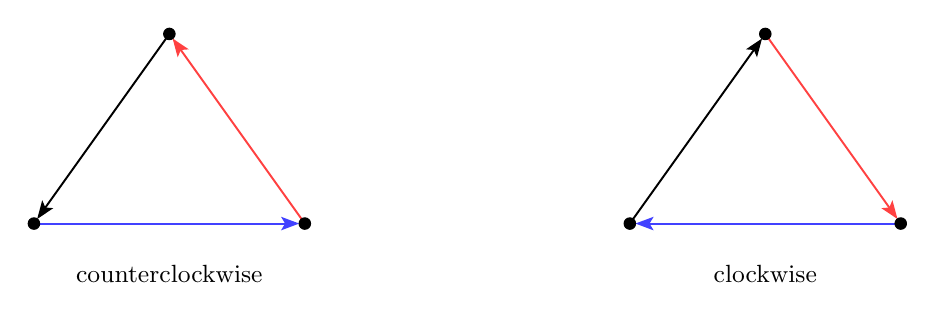
\begin{tikzpicture}[
  scale=1.72,
  >={Stealth[length=2.3mm,width=1.7mm,inset=0.5mm]},
  line cap=round,
  line join=round,
  every node/.style={font=\small}
]
  % Counterclockwise tri-colored face: a -> b -> c -> a (interior on left)
  \begin{scope}[xshift=-2.2cm]
    \coordinate (a) at (-1, 0);
    \coordinate (b) at ( 1, 0);
    \coordinate (c) at ( 0, 1.4);
    \draw[->, line width=0.7pt, ColZero, shorten >=2pt] (a) -- (b);
    \draw[->, line width=0.7pt, ColOne,  shorten >=2pt] (b) -- (c);
    \draw[->, line width=0.7pt, ColTwo,  shorten >=2pt] (c) -- (a);
    \foreach \pt in {a,b,c}{\filldraw[fill=black] (\pt) circle (1.2pt);}
    \node[below=4pt] at (0,-0.15) {counterclockwise};
  \end{scope}

  % Clockwise tri-colored face: b -> a -> c -> b (interior on right)
  \begin{scope}[xshift=2.2cm]
    \coordinate (a) at (-1, 0);
    \coordinate (b) at ( 1, 0);
    \coordinate (c) at ( 0, 1.4);
    \draw[->, line width=0.7pt, ColZero, shorten >=2pt] (b) -- (a);
    \draw[->, line width=0.7pt, ColTwo,  shorten >=2pt] (a) -- (c);
    \draw[->, line width=0.7pt, ColOne,  shorten >=2pt] (c) -- (b);
    \foreach \pt in {a,b,c}{\filldraw[fill=black] (\pt) circle (1.2pt);}
    \node[below=4pt] at (0,-0.15) {clockwise};
  \end{scope}
\end{tikzpicture}
\caption{The two orientations of a tri-colored face.}
\label{fig:tricolored-orientations}
\end{figure}

\begin{lemma}
\label{lem:tricolored-edge-disjoint}
Two tri-colored faces of the same orientation cannot share an edge.
\end{lemma}

\begin{proof}
Suppose two same-oriented tri-colored faces share an edge $e$. Traversing the boundary of each face in its orientation direction traverses $e$ in opposite directions, since the two faces lie on opposite sides of $e$. But $e$ is directed only one way, so it cannot be traversed in both directions.
\end{proof}

\begin{figure}[H]
\centering
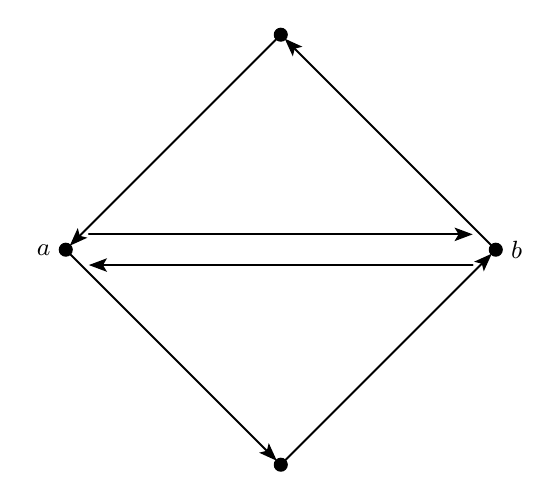
\begin{tikzpicture}[
  scale=1.95,
  >={Stealth[length=2.3mm,width=1.7mm,inset=0.5mm]},
  line cap=round,
  line join=round,
  every node/.style={font=\small}
]
  \coordinate (a) at (-1.4, 0);
  \coordinate (b) at ( 1.4, 0);
  \coordinate (c) at ( 0  , 1.4);
  \coordinate (d) at ( 0  ,-1.4);

  % Upper triangle CCW: b -> c, c -> a
  \draw[->, line width=0.7pt, shorten >=2pt] (b) -- (c);
  \draw[->, line width=0.7pt, shorten >=2pt] (c) -- (a);
  % Lower triangle CCW: a -> d, d -> b
  \draw[->, line width=0.7pt, shorten >=2pt] (a) -- (d);
  \draw[->, line width=0.7pt, shorten >=2pt] (d) -- (b);

  % Shared edge: two conflicting arrows on opposite sides
  \draw[->, line width=0.7pt] ($(a)+(0.15, 0.1)$) -- ($(b)+(-0.15, 0.1)$);
  \draw[->, line width=0.7pt] ($(b)+(-0.15,-0.1)$) -- ($(a)+(0.15,-0.1)$);

  \foreach \pt in {a,b,c,d}{\filldraw[fill=black] (\pt) circle (1.2pt);}
  \node[left=2pt]  at (a) {$a$};
  \node[right=2pt] at (b) {$b$};
\end{tikzpicture}
\caption{Two same-oriented faces force opposite directions on $ab$.}
\label{fig:edge-disjoint-contradiction}
\end{figure}

\begin{proposition}
\label{prop:general-source-bound}
Let $G$ be a simple toroidal triangulation with $n$ vertices, equipped with any local toroidal Schnyder orientation. Then
\[
  \sum_{i \in \Zthree} z_i \;\geq\; n - \Delta^-.
\]
\end{proposition}

\begin{proof}
By Lemma~\ref{lem:tricolored-edge-disjoint}, the counterclockwise-oriented tri-colored faces are pairwise edge-disjoint, so
\[
  3 \Delta^+ \;\leq\; m \;=\; 3n,
\]
and hence $\Delta^+ \leq n$. By Lemma~\ref{lem:tricolored-directed}, $\Delta = \Delta^+ + \Delta^- \leq n + \Delta^-$, and by Corollary~\ref{cor:toroidal-total-source},
\[
  \sum_{i \in \Zthree} z_i \;=\; 2n - \Delta \;\geq\; n - \Delta^-. \qedhere
\]
\end{proof}

We apply Proposition~\ref{prop:general-source-bound} to the minimal Schnyder woods on $G$, that is, to the minimal elements of the distributive lattice of balanced toroidal Schnyder woods studied in~\cite{despre-goncalves-leveque2017}. By the lattice description of that reference, any such minimal Schnyder wood satisfies $\Delta^- \leq 1$.

\begin{theorem}
\label{thm:toroidal-lower-bound}
Let \(G\) be a simple toroidal triangulation with \(n\) vertices, and let \(S\)
be a minimal Schnyder wood on \(G\). Then
\[
  \sum_{i\in\Zthree} z_i \geq \frac{6n-6}{5}.
\]
\end{theorem}
\begin{proof}
By Corollary~\ref{cor:toroidal-total-source},
\[
  \sum_{i\in\Zthree} z_i = 2n-\Delta.
\]
It is therefore enough to prove
\[
  \Delta \leq \frac{4n+6}{5}.
\]

By Lemma~\ref{lem:tricolored-edge-disjoint}, the counterclockwise tri-colored faces
are pairwise edge-disjoint. Hence they use exactly \(3\Delta^+\) distinct edges.

Let \(U\) be the set of edges not used by any counterclockwise tri-colored face. Since
\(|E(G)|=3n\), we have
\[
  |U|=3n-3\Delta^+=3(n-\Delta^+).
\]

Consider a face which is not counterclockwise tri-colored. If none of its boundary
edges belongs to \(U\), then each of its boundary edges is used by a counterclockwise
tri-colored face on the other side. Hence this face lies on the right of each of its
boundary edges, so it is a clockwise directed triangle. By Lemma~\ref{lem:separation},
such a directed facial triangle is necessarily tri-colored. Therefore it is counted by
\(\Delta^-\).

Since \(\Delta^-\leq 1\), among the \(2n-\Delta^+\) faces which are not
counterclockwise tri-colored, all but at most one must be incident with an edge of
\(U\). Each edge of \(U\) is incident with at most two faces, so the number of such
faces is at most \(2|U|\). Thus
\[
  2n-\Delta^+-1 \leq 2|U|=6(n-\Delta^+).
\]
Hence
\[
  \Delta^+\leq \frac{4n+1}{5}.
\]
Thus, we obtain
\[
  \Delta
  =
  \Delta^+ + \Delta^-
  \leq
  \frac{4n+1}{5}+1
  =
  \frac{4n+6}{5}.
\]
Consequently,
\[
  \sum_{i\in\Zthree} z_i
  =
  2n-\Delta
  \geq
  2n-\frac{4n+6}{5}
  =
  \frac{6n-6}{5}.
\]
\end{proof}




\section{Balanced Schnyder woods and oriented triangles}
\label{sec:balanced-triangles}

The preceding sections studied consequences of the local Schnyder rule: the planar leaf--face identity, the toroidal source--face identity, and the resulting lower bound on the source counts of a minimal toroidal Schnyder wood. We now turn to a different kind of statement, where the local rule alone is not enough and a global condition is needed. In this section, unlike in the purely local sections above, we work with toroidal Schnyder woods in the standard global sense, and more specifically with the balanced, or $\gamma_0$, ones. For toroidal triangulations, this is the same class as the HTC Schnyder woods of Despr\'e, Gon\c{c}alves, and L\'ev\^eque, and this class satisfies the dual-acyclicity property needed below.

For this section, fix an orientation of the torus. Each vertex has three outgoing directed colored copies, giving $3n$ in total, while a doubled edge would contribute two outgoing copies and a singly-directed edge one; since $m = 3n$ for a toroidal triangulation, no edge of $G$ is doubled, and the underlying orientation $D$ is an ordinary orientation of the edge set. If $e = u \to v$ is a directed edge, let $F_L(e)$ and $F_R(e)$ be the faces on the left and on the right of $e$, respectively. The dual edge $e^*$ is oriented from $F_L(e)$ to $F_R(e)$; the resulting dual orientation is denoted by $D^*$.

For a non-contractible cycle $C$, oriented arbitrarily, let
\[
  \gamma(C) :=
  \#\{\text{edges leaving $C$ on the right}\}
  - \#\{\text{edges leaving $C$ on the left}\}.
\]
Reversing the orientation of $C$ merely changes the sign of $\gamma(C)$. Thus the condition $\gamma(C) = 0$ is independent of the chosen orientation of $C$.

A toroidal Schnyder wood is called \emph{balanced} if
\[
  \gamma(C) = 0
\]
for every non-contractible cycle $C$. This is the $\gamma_0$ property. In the triangulated case, Despr\'e, Gon\c{c}alves, and L\'ev\^eque recall that the $\gamma_0$ property characterizes the HTC Schnyder woods, as a consequence of the homology classification of Schnyder orientations in \cite[Theorem~3.7 and Section~5.2]{goncalves-knauer-leveque2019}; see also \cite[Section~9]{despre-goncalves-leveque2017}. Moreover, for an HTC Schnyder wood, the dual orientation $D^*$ contains no directed non-contractible cycle \cite[Lemma~2]{despre-goncalves-leveque2017}.

A \emph{directed triangle} is a directed closed walk of length three whose three vertices are distinct. It is \emph{contractible} if its image on the torus can be continuously shrunk to a point, equivalently if it bounds a topological $2$-disk. It is called counterclockwise, respectively clockwise, if this disk lies locally on its left, respectively on its right.

The following theorem is known in this setting \cite[Section~10]{despre-goncalves-leveque2017}. We give a direct proof using only the dual-acyclicity input stated above.

\begin{theorem}
\label{thm:balanced-oriented-triangles}
Every balanced toroidal Schnyder wood on a simple toroidal triangulation contains at least one counterclockwise oriented contractible triangle and at least one clockwise oriented contractible triangle.
\end{theorem}

\begin{proof}
We prove the counterclockwise case in detail. The clockwise case is obtained by performing the following three symmetric replacements throughout: left successors are replaced by right successors, sweeps through the left sector at each vertex are replaced by sweeps through the right sector, and the edge-connected component of \emph{maximum}-label faces is replaced by the edge-connected component of \emph{minimum}-label faces.

Let $D$ be the underlying orientation. If $e = u \to v$ is a directed edge entering $v$, define $L(e)$ as follows. Starting from the edge-end of $e$ at $v$, move in the cyclic order around $v$ through the side locally lying to the left of $e$, and stop at the first outgoing edge encountered. This edge exists because $v$ has exactly three outgoing edges. It is called the \emph{left successor} of $e$. By definition, the open sector from $e$ to $L(e)$ on the left side of $e$ contains no outgoing edge.

\begin{figure}[ht]
\centering
\begin{tikzpicture}[
  scale=1.9,
  >={Stealth[length=2.4mm,width=1.8mm,inset=0.5mm]},
  line cap=round,
  line join=round,
  every node/.style={font=\small}
]
  \coordinate (v) at (0,0);

  % Edge endpoints
  \coordinate (a) at (-2.4,-0.9);
  \coordinate (b) at ( 2.5, 0.55);

  % Other incoming edges in the open left sector
  \coordinate (c) at (-1.9, 1.55);
  \coordinate (d) at (-0.15,2.05);
  \coordinate (e) at ( 1.65,1.50);

  % Other incoming edges (dashed, lighter)
  \draw[->, dashed, gray!70, line width=0.5pt, shorten >=2pt] (c) -- (v);
  \draw[->, dashed, gray!70, line width=0.5pt, shorten >=2pt] (d) -- (v);
  \draw[->, dashed, gray!70, line width=0.5pt, shorten >=2pt] (e) -- (v);

  % Featured edges e_t and e_{t+1}=L(e_t)
  \draw[->, line width=0.9pt, shorten >=2pt] (a) -- (v);
  \draw[->, line width=0.9pt, shorten <=2pt] (v) -- (b);

  % Sweep arc indicating the direction from e_t to L(e_t) through the left side
  \draw[->, gray!65, line width=0.55pt]
    (200:0.85) arc[start angle=200, end angle=15, radius=0.85];

  \filldraw[fill=black] (v) circle (1.4pt);

  % Labels
  \node[below left]  at (-1.55,-0.7) {$e_t$};
  \node[above right] at ( 1.95, 0.55) {$L(e_t)$};
  \node[below=2pt] at (v) {$v$};
\end{tikzpicture}
\caption{The left successor $L(e_t)$ of $e_t$ at $v$.}
\label{fig:left-successor}
\end{figure}

Starting from an arbitrary directed edge $e_0$, define
\[
  e_{t+1} = L(e_t).
\]
Since the graph has finitely many directed edges, this sequence is eventually periodic. Choose one periodic orbit of minimal period and write it as
\[
  W = e_0 e_1 \cdots e_{p-1},
\]
with indices taken modulo $p$. Then $W$ is a directed closed walk, and the directed edges $e_0, \dots, e_{p-1}$ are pairwise distinct.

At the vertex where $e_t$ enters and $e_{t+1}$ leaves, the open left sector between $e_t$ and $e_{t+1}$ contains no outgoing edge, as in Figure~\ref{fig:left-successor}. Thus every edge-end strictly inside this sector is an edge directed toward that vertex.

We first prove that $W$ is contractible. Let $v_t$ be the vertex where $e_t$ enters and $e_{t+1}$ leaves, and set $L_t = F_L(e_t)$. In the left sector at $v_t$, the consecutive faces from $L_t$ to $L_{t+1}$ are separated by edges directed toward $v_t$. With the convention that a dual edge is directed from the left face of a primal edge to its right face, the corresponding dual edges form a directed dual path from $L_{t+1}$ to $L_t$. Concatenating these paths in the order
\[
  L_0 \to L_{p-1} \to L_{p-2} \to \cdots \to L_1 \to L_0
\]
gives a directed closed dual walk, denoted \emph{the left-sector dual walk} $W_L^*$. The local construction is illustrated in Figure~\ref{fig:left-dual-path}. Note that, since each local dual path runs from $L_{t+1}$ back to $L_t$, $W_L^*$ traverses its image in the direction opposite to that of $W$ on the primal.

\begin{figure}[ht]
\centering
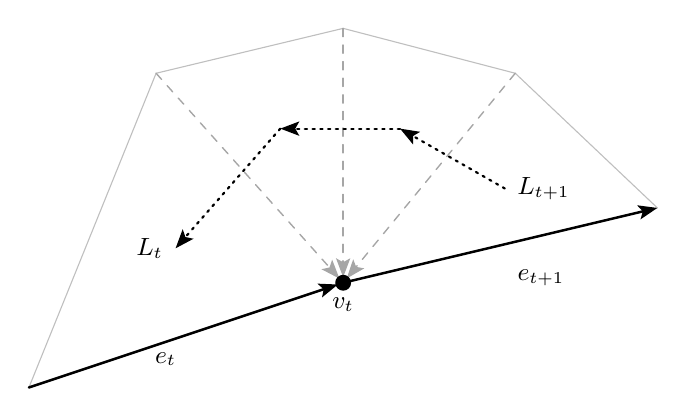
\begin{tikzpicture}[
  scale=1.9,
  >={Stealth[length=2.4mm,width=1.8mm,inset=0.5mm]},
  line cap=round,
  line join=round,
  every node/.style={font=\small}
]
  \coordinate (v) at (0,0);

  \coordinate (a) at (-2.1,-0.7);
  \coordinate (b) at ( 2.1, 0.5);
  \coordinate (c) at (-1.25,1.4);
  \coordinate (d) at ( 0.0 ,1.7);
  \coordinate (e) at ( 1.15,1.4);

  % Face centers (centroids), close to v
  \coordinate (Lt)  at (-1.12, 0.23);
  \coordinate (G1)  at (-0.42, 1.03);
  \coordinate (G2)  at ( 0.38, 1.03);
  \coordinate (Ltp) at ( 1.08, 0.63);

  % Triangulation edges (light grey)
  \draw[gray!50, line width=0.4pt] (a) -- (c);
  \draw[gray!50, line width=0.4pt] (c) -- (d);
  \draw[gray!50, line width=0.4pt] (d) -- (e);
  \draw[gray!50, line width=0.4pt] (e) -- (b);

  % Other incoming primal edges (dashed)
  \draw[->, dashed, gray!70, line width=0.5pt, shorten >=2pt] (c) -- (v);
  \draw[->, dashed, gray!70, line width=0.5pt, shorten >=2pt] (d) -- (v);
  \draw[->, dashed, gray!70, line width=0.5pt, shorten >=2pt] (e) -- (v);

  % Featured primal edges
  \draw[->, line width=0.9pt, shorten >=2pt] (a) -- (v);
  \draw[->, line width=0.9pt, shorten <=2pt] (v) -- (b);

  % Dual walk: dotted arrows through face centers, from L_{t+1} to L_t
  \draw[->, line width=0.8pt, dotted] (Ltp) -- (G2);
  \draw[->, line width=0.8pt, dotted] (G2) -- (G1);
  \draw[->, line width=0.8pt, dotted] (G1) -- (Lt);

  % Vertex v_t
  \filldraw[fill=black] (v) circle (1.4pt);

  % Labels
  \node[below left]  at (-1.05,-0.4) {$e_t$};
  \node[below right] at ( 1.1, 0.15) {$e_{t+1}$};
  \node[below=2pt] at (v) {$v_t$};
  \node[left=1pt]   at (Lt)  {$L_t$};
  \node[right=1pt]  at (Ltp) {$L_{t+1}$};
\end{tikzpicture}
\caption{The left-sector dual walk from $L_{t+1}$ to $L_t$.}
\label{fig:left-dual-path}
\end{figure}

We now compare the contractibility of $W$ and $W_L^*$. Since dual edges are drawn inside the faces they cross, we may choose their drawings freely inside those faces. We draw each dual path used in the construction of $W_L^*$ inside a sufficiently thin neighborhood of the corresponding part of $W$, always on the left side of $W$. With this choice, the drawn copy of $W_L^*$ is a left parallel copy of $W$, with only small detours inside the faces incident with $W$.

Thus $W$ and the drawn copy of $W_L^*$ lie in the same thin neighborhood of $W$, and this neighborhood has two boundary walks which run parallel to one another. Moving from one boundary walk to the other inside the neighborhood does not change whether the walk is contractible: a closed walk contained in such a neighborhood wraps around the torus exactly when any sufficiently close parallel copy does. Reversing the direction of traversal also preserves contractibility. Hence $W$ is contractible if and only if $W_L^*$ is contractible.

If $W$ were non-contractible, then $W_L^*$ would be a non-contractible directed closed dual walk. By the fact recalled in Section~\ref{sec:prelim}, such a walk contains a directed non-contractible dual cycle. This contradicts the dual-acyclicity property above. Therefore $W$ is contractible.

We now define an integer label on the faces. Fix
\[
  Q_0 := F_R(e_0)
\]
and set $\lambda(Q_0) = 0$. For any face $F$, choose a dual walk from $Q_0$ to $F$. Along this walk, crossing an edge not in $W$ does not change the label; crossing an edge of $W$ from right to left adds $1$, and crossing an edge of $W$ from left to right subtracts $1$.

This label is well-defined. Indeed, two choices of dual walk differ by a closed dual walk, and the total change of the label along such a closed dual walk is its signed number of crossings with $W$. Since $W$ is contractible, it is null-homologous on the torus, and the algebraic intersection number of a null-homologous $1$-cycle with any other $1$-cycle is zero. Hence the right-to-left and left-to-right crossings cancel, and the value of $\lambda(F)$ is independent of the chosen dual walk. Consequently, for every directed edge $e$,
\begin{equation}
\label{eq:label-jump}
\lambda(F_L(e)) - \lambda(F_R(e))
=
\begin{cases}
1, & \text{if } e \text{ occurs in } W,\\
0, & \text{if } e \text{ does not occur in } W.
\end{cases}
\end{equation}

Let
\[
  M = \max_F \lambda(F).
\]

By an \emph{edge-connected component} of a set of faces we mean a maximal subset in which any two faces are joined by a sequence of pairwise edge-adjacent faces from the subset, where two faces are edge-adjacent when they share a primal edge of $G$. Choose one edge-connected component of the set of faces with label $M$. From this component we build an abstract region $R$: take one copy of each face in the component, and glue two copies along an edge precisely when the corresponding faces of $G$ share that edge. If the same vertex of $G$ appears several times on the boundary, these appearances are kept as distinct boundary occurrences. Thus $R$ is a compact connected orientable surface with non-empty boundary, made of triangular faces, and it maps naturally to $G$.

Every boundary edge of $R$ maps to an edge of $W$, directed with $R$ on its left. To see this, let $a$ be a boundary edge of $R$. The face of $R$ incident with $a$ has label $M$. The face on the other side of $a$ cannot also have label $M$, otherwise it would belong to the same edge-connected component. Thus the label changes across $a$. By \eqref{eq:label-jump}, the edge $a$ must map to an edge of $W$. Moreover, the side of label $M$ is the left side of this directed edge, because the label increases by one from right to left across an edge of $W$.

We next prove that no boundary occurrence of $R$ has an outgoing edge strictly inside $R$. Let $x$ be a boundary occurrence, and let $v$ be its image in $G$. Let $\hat e$ and $\hat f$ be the boundary edges entering and leaving $x$, and let $e$ and $f$ be their images in $G$. By the previous paragraph, $e$ and $f$ are edges of $W$, directed with $R$ on their left. Therefore the sector of $R$ at $x$ is contained in the left sector of $e$, and $f$ is an outgoing edge in that sector.

Since the next edge of $W$ after $e$ is $L(e)$, and since $L(e)$ is the first outgoing edge in the left sector of $e$, the edge $L(e)$ is encountered no later than $f$ when one sweeps through this sector. If $L(e) \neq f$, then $L(e)$ lies strictly inside the sector of $R$ at $x$. The two face occurrences adjacent to $L(e)$ at $x$ would then both belong to $R$, and hence both would have label $M$. But $L(e)$ is an edge of $W$, so \eqref{eq:label-jump} says that the labels on its two sides differ by $1$, a contradiction. Thus $f = L(e)$. Since the open sector from $e$ to $L(e)$ contains no outgoing edge, there is no outgoing edge from the boundary occurrence $x$ strictly into $R$.

\begin{figure}[ht]
\centering
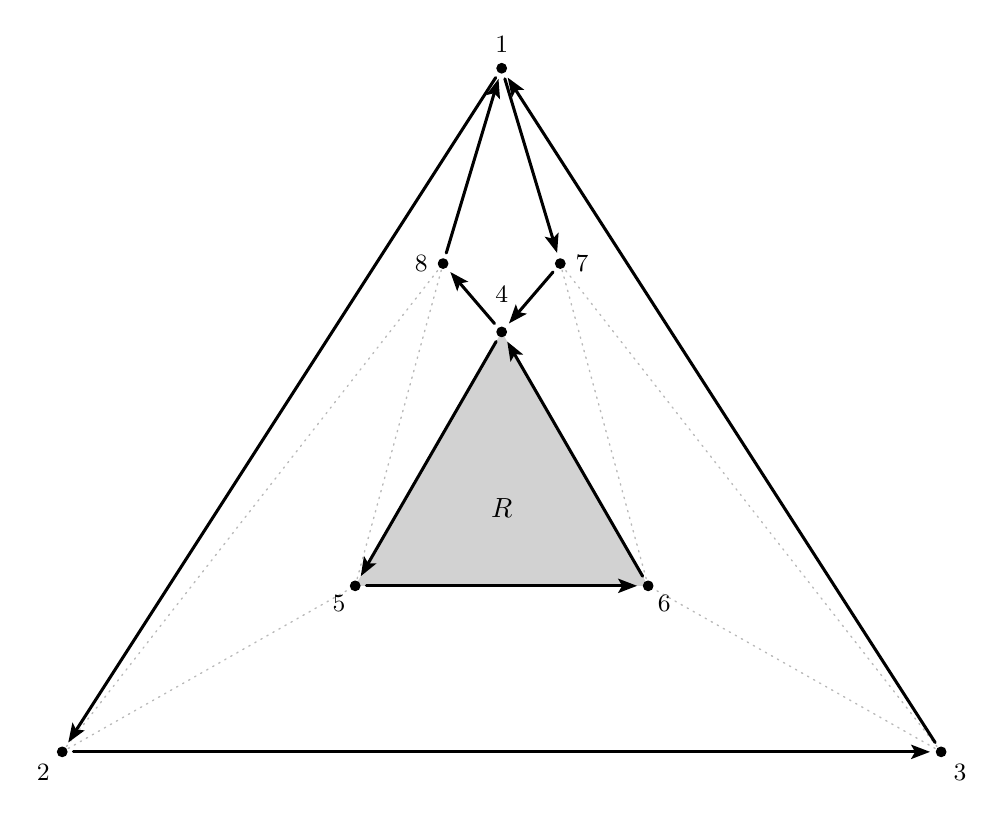
\begin{tikzpicture}[
  scale=1.24,
  >={Stealth[length=2.4mm,width=1.8mm,inset=0.5mm]},
  line cap=round,
  line join=round,
  every node/.style={font=\small}
]
  % Outer triangle (CCW: 1 -> 2 -> 3 -> 1)
  \coordinate (v1) at ( 0  , 4.5);
  \coordinate (v2) at (-4.5,-2.5);
  \coordinate (v3) at ( 4.5,-2.5);

  % Inner triangle (CCW: 4 -> 5 -> 6 -> 4), boundary of R
  \coordinate (v4) at ( 0  , 1.8);
  \coordinate (v5) at (-1.5,-0.8);
  \coordinate (v6) at ( 1.5,-0.8);

  % Internal vertices of the two paths (pulled away from outer edges)
  \coordinate (v7) at ( 0.6, 2.5);
  \coordinate (v8) at (-0.6, 2.5);

  % R = interior of inner triangle (only shaded region)
  \fill[gray!35] (v4) -- (v5) -- (v6) -- cycle;

  % Auxiliary triangulation edges (faint dotted; not part of W)
  \draw[gray!55, dotted, line width=0.5pt] (v2) -- (v5);
  \draw[gray!55, dotted, line width=0.5pt] (v3) -- (v6);
  \draw[gray!55, dotted, line width=0.5pt] (v3) -- (v7);
  \draw[gray!55, dotted, line width=0.5pt] (v2) -- (v8);
  \draw[gray!55, dotted, line width=0.5pt] (v7) -- (v6);
  \draw[gray!55, dotted, line width=0.5pt] (v8) -- (v5);

  % Walk W (heavy arrows): 1 -> 2 -> 3 -> 1 -> 7 -> 4 -> 5 -> 6 -> 4 -> 8 -> 1
  \draw[->, line width=1.1pt, shorten >=4pt, shorten <=4pt] (v1) -- (v2);
  \draw[->, line width=1.1pt, shorten >=4pt, shorten <=4pt] (v2) -- (v3);
  \draw[->, line width=1.1pt, shorten >=4pt, shorten <=4pt] (v3) -- (v1);
  \draw[->, line width=1.1pt, shorten >=4pt, shorten <=4pt] (v1) -- (v7);
  \draw[->, line width=1.1pt, shorten >=4pt, shorten <=4pt] (v7) -- (v4);
  \draw[->, line width=1.1pt, shorten >=4pt, shorten <=4pt] (v4) -- (v5);
  \draw[->, line width=1.1pt, shorten >=4pt, shorten <=4pt] (v5) -- (v6);
  \draw[->, line width=1.1pt, shorten >=4pt, shorten <=4pt] (v6) -- (v4);
  \draw[->, line width=1.1pt, shorten >=4pt, shorten <=4pt] (v4) -- (v8);
  \draw[->, line width=1.1pt, shorten >=4pt, shorten <=4pt] (v8) -- (v1);

  % Vertex dots
  \foreach \pt in {v1, v2, v3, v4, v5, v6, v7, v8}{
    \filldraw[fill=black] (\pt) circle (1.4pt);
  }

  % Vertex labels
  \node[above=2pt]       at (v1) {$1$};
  \node[below left=1pt]  at (v2) {$2$};
  \node[below right=1pt] at (v3) {$3$};
  \node                  at ( 0.0, 2.18) {$4$};
  \node[below left=0pt]  at (v5) {$5$};
  \node[below right=0pt] at (v6) {$6$};
  \node[right=2pt]       at (v7) {$7$};
  \node[left=2pt]        at (v8) {$8$};

  % R label inside the shaded region
  \node[font=\itshape] at ( 0.0, 0.0) {$R$};
\end{tikzpicture}
\caption{The walk $W$ (1-2-3-1-7-4-5-6-4-8-1) and the depth-$2$ region $R$ (shaded).}
\label{fig:max-label-region}
\end{figure}

It remains to count inside $R$. Vertices and edges are now understood as cells of the abstract surface $R$, not as vertices and edges of $G$. In particular, repeated boundary appearances of the same vertex of $G$ are counted as distinct boundary vertices of $R$. Let
\[
  n_R = \#V(R), \qquad m_R = \#E(R), \qquad f_R = \#F(R),
\]
and let $K_R$ be the total boundary length of $R$. With the above convention, $K_R$ is also the number of boundary vertex occurrences of $R$.

Counting edges of $R$ by their tails gives
\begin{equation}
\label{eq:tail-count-R}
  m_R = 3(n_R - K_R) + K_R = 3 n_R - 2 K_R.
\end{equation}
Indeed, an interior vertex occurrence of $R$ has all its incident face occurrences in $R$, so all three outgoing edges at that occurrence are edges of $R$. At a boundary vertex occurrence, the previous paragraph shows that there is no outgoing edge strictly inside the sector of $R$. Hence the only outgoing edge of $R$ at that boundary occurrence is the boundary edge leaving that occurrence. Since boundary occurrences are counted separately, this contributes exactly one outgoing edge for each of the $K_R$ boundary vertex occurrences.

Let $g$ be the genus of $R$, and let $b$ be the number of boundary components. Then
\[
  \chi(R) = 2 - 2g - b.
\]
Euler's formula and the triangular face count give
\[
  n_R - m_R + f_R = \chi(R),
  \qquad
  3 f_R = 2 m_R - K_R.
\]
Substituting $f_R = \chi(R) - n_R + m_R$ into $3 f_R = 2 m_R - K_R$ yields
\begin{equation}
\label{eq:euler-count-R}
  m_R = 3 n_R - K_R - 3 \chi(R).
\end{equation}
Comparing \eqref{eq:tail-count-R} and \eqref{eq:euler-count-R}, we obtain
\[
  K_R = 3 \chi(R).
\]

Moreover $R$ is not the whole torus, since $Q_0 = F_R(e_0)$ has label $0$ while $L_0 = F_L(e_0)$ has label $1$. Hence the boundary of $R$ is non-empty, so $K_R > 0$ and hence $\chi(R) > 0$. Since $\chi(R) = 2 - 2g - b$ with $g \ge 0$ and $b \ge 1$, the only possibility is $g = 0$ and $b = 1$. Thus $R$ is a topological disk and $\chi(R) = 1$. Therefore $K_R = 3$.

Thus $\partial R$ has exactly three directed boundary edge occurrences. Each boundary edge occurrence of $R$ maps to an edge of $W$, directed with $R$ on its left. Moreover, the three image edges in $G$ are distinct: a directed edge of $W$ has a unique face on its left, and a face copy of $R$ is included only once in the chosen edge-connected component of maximum-label faces. Hence the image of $\partial R$ in $G$ is a directed closed walk of length three, supported by three distinct directed edges of the original Schnyder wood. Its three vertices are distinct; otherwise $G$ would contain a loop or two parallel edges. Hence this walk is a genuine directed triangle.

The region $R$ is a disk bounded by this triangle, so the triangle is contractible. Since $R$ lies on the left of each boundary edge, the triangle is counterclockwise.
\end{proof}


\section{Concluding remarks}
\label{sec:conclusion}

\begingroup
\renewcommand{\addcontentsline}[3]{}

\subsection*{Summary}
The results of this paper are organized around a single question: to what extent is the structure of a Schnyder wood determined by the local rule satisfied at each vertex, and at which point does a global hypothesis become indispensable?

Two of the results show that the local rule alone determines a great deal. In the plane it yields the leaf--face identity $\sum_{i} l_i = 2n + 1 - \kappa$, relating the total number of leaves of the three rooted trees to a single face statistic. On the torus, where the rooted trees become monochromatic functional digraphs and the leaves become sources, the same rule yields a parallel source--face identity, and from it the linear bound $\sum_i z_i \geq \frac{6n-6}{5}$ for a minimal Schnyder wood. The two identities are thus instances of a single local phenomenon, the sources on the torus playing the role of the leaves in the plane.

The third result delimits the reach of such local reasoning. The existence of a clockwise and a counterclockwise oriented contractible triangle in every balanced wood does not follow from the local rule alone; it depends on the global hypothesis of balancedness, through the dual-acyclicity it entails, which is what allows a leftmost walk to bound a genuine region and makes the face labeling consistent. The two parts of the paper therefore delimit, from either side, the boundary between what the local rule determines on its own and what only a global condition can ensure.

\subsection*{Outlook}
Several questions remain open. The most immediate one is quantitative: there is no evident structural reason why the planar and toroidal settings should differ substantially in the number of sources that a Schnyder wood must contain. In the planar triangulated case, the leaf count is at least \((3n+3)/2\), whereas the present toroidal argument gives only
\(
\sum_i z_i \geq \frac{6n-6}{5}.
\)
It is therefore natural to ask for the sharp lower bound on the number of sources in minimal toroidal Schnyder woods. The gap is likely due to the method of proof rather than to the underlying structure: the present argument uses only a coarse edge-disjointness count for tri-colored faces, thereby ignoring much of the finer combinatorial information carried by the Schnyder wood.

A second question is whether the same phenomenon persists in higher genus. The source--face identity is purely local and should remain valid on a triangulation of any genus, yielding an analogous bound there. Indeed, the identity $z_i = A_i$ and the edge-disjointness of equally oriented tri-colored faces carry over without change for $g \geq 1$; what does not extend is the global input controlling the clockwise faces. The principal obstacle is thus to identify a higher-genus substitute for the bound on $\Delta^-$.

The same boundary recurs for the oriented-triangle theorem, where one would expect contractible triangles of both orientations on a surface of any genus. The leftmost-walk and Euler-counting argument appears robust, but it relies on two features specific to the torus: the dual-acyclicity of balanced woods, and the fact that a contractible closed walk is null-homologous, which makes the face label well-defined. Its extension would require higher-genus analogues of both, the homological ingredient being the genuine obstacle.

Special thanks to Prof. Castelli Aleardi for introducing me to this wonderful topic.
\endgroup

\newpage
\begin{thebibliography}{10}

\bibitem{castelli-fusy-lewiner2009}
L.~Castelli Aleardi, \'E.~Fusy, and T.~Lewiner.
\newblock Schnyder woods for higher genus triangulated surfaces, with
  applications to encoding.
\newblock {\em Discrete \& Computational Geometry}, 42(3):489--516, 2009.

\bibitem{despre-goncalves-leveque2017}
V.~Despr\'e, D.~Gon\c{c}alves, and B.~L\'ev\^eque.
\newblock Encoding toroidal triangulations.
\newblock {\em Discrete \& Computational Geometry}, 57(3):507--544, 2017.

\bibitem{felsner2001}
S.~Felsner.
\newblock Convex drawings of planar graphs and the order dimension of
  $3$-polytopes.
\newblock {\em Order}, 18(1):19--37, 2001.

\bibitem{felsner2004}
S.~Felsner.
\newblock Lattice structures from planar graphs.
\newblock {\em Electronic Journal of Combinatorics}, 11(1):\#R15, 2004.

\bibitem{goncalves-knauer-leveque2019}
D.~Gon\c{c}alves, K.~Knauer, and B.~L\'ev\^eque.
\newblock On the structure of Schnyder woods on orientable surfaces.
\newblock {\em Journal of Computational Geometry}, 10(1):127--163, 2019.

\bibitem{goncalves-leveque2014}
D.~Gon\c{c}alves and B.~L\'ev\^eque.
\newblock Toroidal maps: Schnyder woods, orthogonal surfaces and straight-line
  representations.
\newblock {\em Discrete \& Computational Geometry}, 51(1):67--131, 2014.

\bibitem{ortlieb-schmidt}
C.~Ortlieb and J.~M. Schmidt.
\newblock Structural parameters of Schnyder woods.
\newblock {\em Discrete Mathematics}, 348(2):114282, 2025.

\bibitem{schnyder1989}
W.~Schnyder.
\newblock Planar graphs and poset dimension.
\newblock {\em Order}, 5(4):323--343, 1989.

\bibitem{schnyder1990}
W.~Schnyder.
\newblock Embedding planar graphs on the grid.
\newblock In {\em Proceedings of the First Annual ACM--SIAM Symposium on
  Discrete Algorithms (SODA)}, pages 138--148, 1990.

\end{thebibliography}

\end{document}